% *******************************************************************
% Setup Document
% *******************************************************************
\documentclass[12pt]{scrbook}
%\documentclass[12pt]{book}
%\documentclass[12pt,openany,oneside]{book}
\usepackage[T1]{fontenc}
\usepackage[ngerman]{babel}
\usepackage{graphicx}
\usepackage{wallpaper}
\usepackage{pdfpages}
\usepackage{fancyhdr}
\usepackage{lastpage}
\usepackage{color}
\usepackage[percent]{overpic}
\usepackage{xcolor}
\usepackage{tikz}
\usepackage[utf8]{inputenc}
\usepackage[update]{epstopdf}
\usepackage{geometry}
\usepackage{epstopdf}
\usepackage[clearempty]{titlesec}
\usepackage{amsmath}
\usepackage{url}
\usepackage{multirow}
\usepackage{paralist}
\usepackage{wrapfig}
\usepackage{colortbl}
\usepackage{makeidx}
\makeindex
\usepackage{array}
\usepackage{textcomp,pifont,wasysym,dingbat,marvosym,skull,amssymb}
\newcolumntype{C}[1]{>{\centering\arraybackslash}p{#1}}
\usepackage[pdftex]{hyperref}
%\usepackage{makeidx}
\usepackage{movie15}
%\epstopdfDeclareGraphicsRule{.gif}{png}{.png}{convert gif:#1 png:\OutputFile}
%\AppendGraphicsExtensions{.gif}

\def\UrlBreaks{\do\a\do\b\do\c\do\d\do\e\do\f\do\g\do\h\do\i\do\j\do\k\do\l%
\do\m\do\n\do\o\do\p\do\q\do\r\do\s\do\t\do\u\do\v\do\w\do\x\do\y\do\z\do\0%
\do\1\do\2\do\3\do\4\do\5\do\6\do\7\do\8\do\9\do\-}%

\geometry{a4paper, left=30mm, right=20mm, top=25mm, bottom=20mm, foot=8mm, headsep=6mm}

% *******************************************************************
%Schriftgroesse der Fussnoten
% *******************************************************************
\def\footnotesize{\fontsize{10pt}{10pt}\selectfont}
\parindent 0pt
% *******************************************************************
% hyperef PDF Setup
% *******************************************************************

\hypersetup {
	colorlinks = {true},
	linkcolor = {black},
	anchorcolor = {black},
	citecolor = {green},
	filecolor = {cyan},
	menucolor = {red},
	urlcolor = {blue},
pdfauthor = {Matthias Ohrt, Adrian Imme und Stefan Nuber}, 
pdftitle = {Erneuerbare Energien}, 
pdfsubject = {Informationen zu Wasserkraft, Windenergie und Solarzellen}, 
pdfstartpage = {1},
}

% *******************************************************************
%Commands
% *******************************************************************
\newcommand{\changefont}[3] {
	\fontfamily{#1}
	\fontseries{#2}
	\fontshape{#3}
	\selectfont
}


\newcommand \leerseite{\newpage\thispagestyle{empty}\hspace{1cm}\newpage}

%\renewcommand{\familydefault}{cmr}
\renewcommand{\familydefault}{ppl}
% *******************************************************************
\setlength{\headheight}{16pt}
%Document

\begin{document}


%Define Header & Footer
\pagestyle{fancy}
\fancyhf{}



%\fancyhead[EL]{\thepage}
%\fancyhead[OR]{\thepage}
\fancyhead[OR]{\leftmark}
\fancyhead[EL]{\rightmark}
%\renewcommand{\headrulewidth}{0.4pt}
\fancyfoot[EL]{\fcolorbox{blue}{gray!20}{Seite: \thepage\ von
\pageref{LastPage}}}
\fancyfoot[OR]{\fcolorbox{blue}{gray!20}{Seite: \thepage\ von
\pageref{LastPage}}}
%\fancyfoot[OL]{Copyright \copyright \ Adrian Imme}
%\fancyfoot[ER]{Copyright \copyright \ Adrian Imme}
\renewcommand{\footrulewidth}{0.4pt}


%\titleformat{\chapter}{\bf\huge}{\thechapter\quad}{-10mm}{}


%%%%%%%%%%%%%%%%%%%%%%%%%%%%%%%%%%%%%%
%%%%%%%%%%Trainer Handout %%%%%%%%%
%%%%%%%%%%%%%%%%%%%%%%%%%%%%%%%%%%%%%%
%Deckblatt
%Deckblatt
\begin{titlepage}
\ThisCenterWallPaper{1}{pictures/deckblatt/ADRIAN_ERNEUERBARE_ENERGIE.pdf}


%
\thispagestyle{empty}
\hbox{ }
\end{titlepage}
\newpage

%Leere Seite nach Titelseite
\thispagestyle{empty}
\cleardoublepage

\newpage
\thispagestyle{empty}

\subject{Ausarbeitung}
\title{Erneuerbare Energien}
\subtitle{Informationen zu Wasserkraft, Windenergie und Solarzellen}
\author{Matthias Ohrt, Adrian Imme und Stefan Nuber}
\date{15. April 2013}
%\publishers{Unterstützt durch Roland Imme}

\maketitle

%\includegraphics[width=1\textwidth]{pictures/bilder/titel.png}

%\newpage

%\thispagestyle{empty}

%Dieses Handout wurde ausschließlich zu Trainingszwecken betreffend der Kaspersky
Lab Software erstellt und stellt keine Produktbeschreibung dar. Die Haftung von
Kaspersky Labs GmbH für etwaige Schäden, die auf irgendeine Art aus der
Benutzung des Handouts entstehen könnten, wird, sofern gesetzlich möglich,
ausgeschlossen. Auch stellen die im Handout getroffenen Aussagen keine
Garantieerklärung der Kaspersky Labs GmbH dar.\\
\\
Die in diesem Handout angegebenen Produktnamen und Beschriftungen können
Handelsmarken Dritter sein.\\
\\
Dieses Handout ist urheberrechtlich geschützt. Alle Rechte sind der Kaspersky
Labs GmbH vorbehalten. Kein Teil des Handouts darf ohne schriftliche Zustimmung
der Kaspersky Labs GmbH in irgendeiner Form (insbesondere Druck, Fotokopie,
Mikrofilm oder einem anderen Verfahren), auch nicht für Zwecke der
Unterrichtsgestaltung, reproduziert, vervielfältigt, verarbeitet, veröffentlicht
oder verbreitet werden.\\
\\
\\
Copyright \copyright \ 2012 Kaspersky Labs GmbH



\vspace*{8cm}
Autoren: Daniel Wischnewski, Peter Aicher und Roland Imme\\
Satz: Roland Imme (\LaTeX)\\
Gesamtgestaltung: Kaspersky Labs GmbH\\


Internet: \url{http://www.kaspersky.com/de/}

\newpage

%\begin{small}
% Inhaltsverzeichnis in den PDF-Links eintragen
\pdfbookmark[1]{Inhaltsverzeichnis}{toc}
\setcounter{tocdepth}{3}
\tableofcontents
\setcounter{secnumdepth}{3}
%\end{small}

\thispagestyle{empty}
\newpage
%%%%%%%%%%%%%%%%%%%%%%%%%%
%%%%%%%%Neue Seite%%%%%%%%
%%%%%%%%%%%%%%%%%%%%%%%%%%

\chapter{Wasserkraft (Matthias Ohrt)}

\begin{figure}[htbp] 
  \centering
     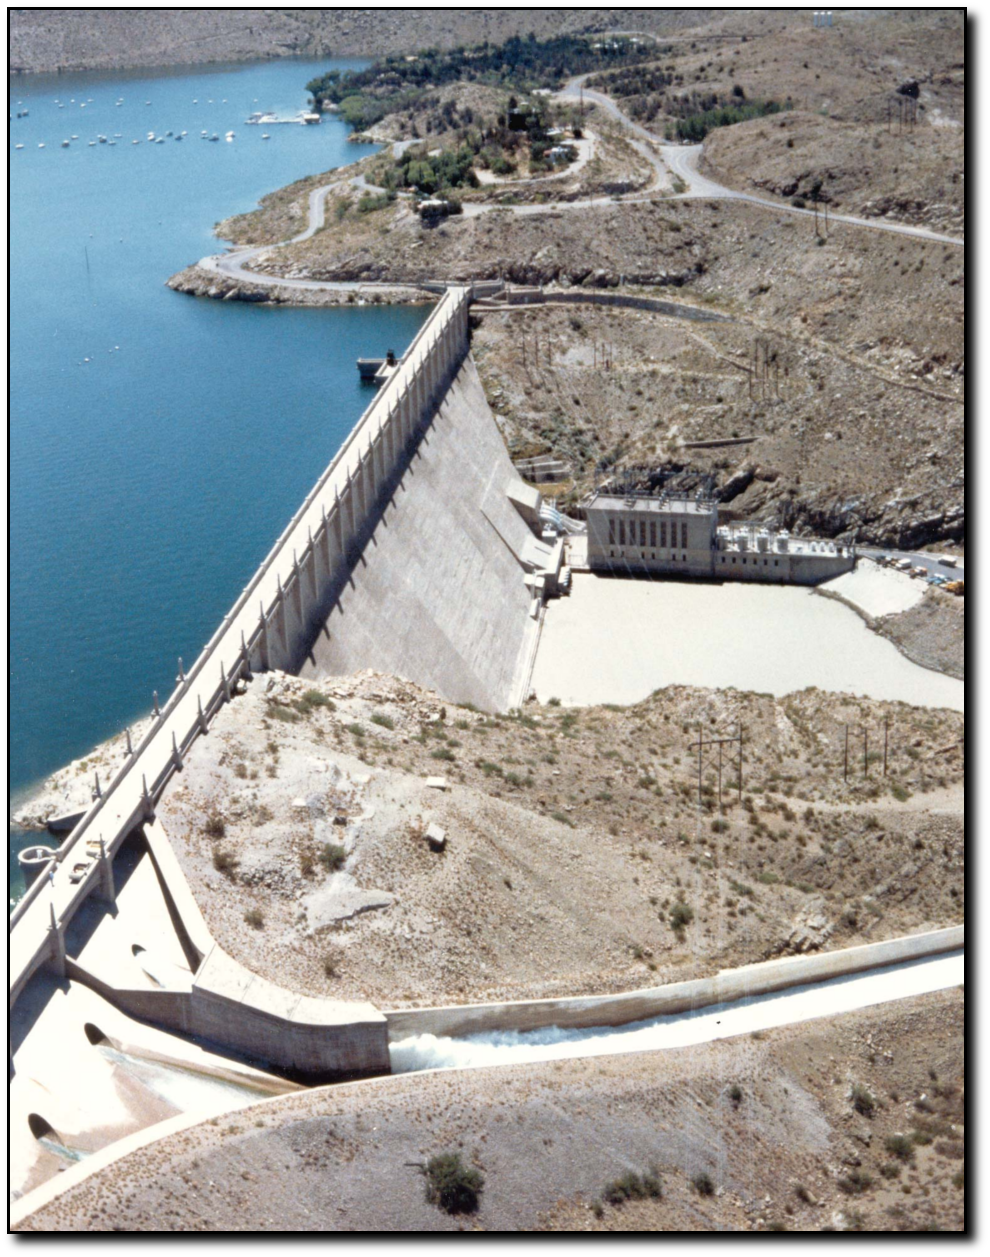
\includegraphics[height=0.7\textheight]{pictures/deckblatt/Elephant_butte_dike.png}
  \caption{Wasserkraftwerk}
  \label{pic:Wasserkraftwerk}
\end{figure}


\newpage
%%%%%%%%%%%%%%%%%%%%%%%%%%
%%%%%%%%Neue Seite%%%%%%%%
%%%%%%%%%%%%%%%%%%%%%%%%%%

\section{Allgemein Informationen}

Die \textsc{Wasserkraft}\index{Wasserkraft} ist eine von vielen sogenannten regenerativen Energien und wurde auch 
schon von den alten Ägyptern vor mehreren tausend Jahren genutzt und viele Jahre später 
im 15. Jahrhundert auch von Müllern um Getreide zu mahlen. Doch heutzutage wird die 
Wasserkraft ausschließlich zur Erzeugung von Strom genutzt. Es gibt viele verschiedene 
Möglichkeiten Wasserkraft zu nutzen, zum Beispiel zur \textsc{Bewässerung}\index{Bewässerung} (wie es die Ägypter 
gemacht haben) oder um Mühlen anzutreiben. Allerdings werden wir uns mit der Erzeugung 
elektrischer Energie mit Hilfe von Wasserkraft befassen. Die Wasserkraft hat zwei bedeutende 
Faktoren die es ermöglichen elektrische Energie zu erzeugen, nämlich die \textsc{Höhen-Bewegungsenergie}\index{Höhen-Bewegungsenergie}. 
Durch diese zwei Formen der Energie ist es möglich in \textsc{Wasserkraftwerken}\index{Wasserkraftwerken} durch verschiedene 
\textsc{Turbinen}\index{Turbinen} Strom zu erzeugen, den wir heute alle nutzen. Doch Wasser kann auch durch andere 
Methoden zur Stromerzeugung genutzt werden. Zum Beispiel in Kohle oder Atomkraftwerken, wo 
das Wasser zum \textsc{Verdampfen}\index{Verdampfen} gebracht wird und schließlich \textsc{Generatoren}\index{Generatoren} antreibt, doch diese Art 
der Stromerzeugung geht in den Bereich der Fossilen Energie, welche in diesem Referat von keiner großen Bedeutung ist.

\newpage
%%%%%%%%%%%%%%%%%%%%%%%%%%
%%%%%%%%Neue Seite%%%%%%%%
%%%%%%%%%%%%%%%%%%%%%%%%%%

\section{Die Francis Turbine}

Sie wurde 1849 von James B. Francis erfunden. Bei der \textsc{Francis Turbine}\index{Francis Turbine} wird das
Wasser durch ein feststehendes Leitrad mit verstellbaren Schaufeln auf die
gegenläufig gekrümmten Schaufeln des Laufrades gelenkt. Da das Wasser vor dem
Eintritt in die Turbine unter höherem Druck steht als nach dem Austritt,
spricht man von einer Überdruckturbine. Dieser Turbinentyp wird in 
\textsc{Laufwasserkraftwerken}\index{Laufwasserkraftwerken}, vor allem aber in Speicher- und 
Pumpspeicherkraftwerken
bei Fallhöhen bis 700 m eingesetzt, wo sie Leistungen bis 750 MW bei einem
Wirkungsgrad bis 90\% erzielen können. Ein Vorteil der Francis Turbine ist,
dass sie auch als Pumpe eingesetzt wird, daher kann sie auch in
Speicherkraftwerken eingesetzt werden.



\newpage
%%%%%%%%%%%%%%%%%%%%%%%%%%
%%%%%%%%Neue Seite%%%%%%%%
%%%%%%%%%%%%%%%%%%%%%%%%%%

\section{Die Kaplanturbine}

1912-1918 entstand diese Turbine durch den Österreicher Victor Kaplan. Diese
Turbinenart gleicht einer Schiffsschraube. Der eintretende Wasserstrom wird
von dem Leitwerk so gelenkt, dass er parallel zur senkrecht angeordneten Welle
auf 3-6 verdrehbare Schaufeln des Laufrades trifft. Die Flügel des
Turbinenlaufrades sind verstellbar. Dadurch kann die Turbinenleistung an das
schwankende Flußwasserangebot angepasst werden. Diese Turbine wird
hauptsächlich bei Fallhöhen von 2-60 m eingesetzt. Sie wird bis zu einer
Leistung von 125 MW gebaut und arbeitet mit einem maximalen Wirkungsgrad von
95\%.


\subsection{Die Kaplan-Rohrturbine}

Aus der \textsc{Kaplan-Turbine}\index{Kaplan-Turbine} wurde für niedrige Fallhöhen (max. 25 m) die
\textsc{Kaplan-Rohrturbine}\index{Kaplan-Rohrturbine} entwickelt, die Leistungen bis zu 75 MW erzielt. Die
Rohr-Turbinen werden, um Umlenkverluste weitgehend zu vermeiden, horizontal in
der Richtung des strömenden Wassers eingebaut. Der Generator befindet sich in
der Verlängerung der Turbinenwelle in einem vom Wasser umströmten,
wasserdichten Gehäuse. Axial durchströmte Rohrturbinen haben mit dem
höheren Vollastwirkungsgrad sowie einer größeren Schluckfähigkeit gegenüber
vertikalen Kaplan-Turbinen vielfache Vorteile. Rohr-Turbinen oder
Horizontalturbinen sparen Platz und ermöglichen geringere Bauhöhen der
Krafthäuser. Dadurch wirken sie weniger störend in der Landschaft. Aus diesem
Grund wurden in letzter Zeit vorwiegend \textsc{Rohr-Turbinen}\index{Rohr-Turbinen} installiert.


\newpage
%%%%%%%%%%%%%%%%%%%%%%%%%%
%%%%%%%%Neue Seite%%%%%%%%
%%%%%%%%%%%%%%%%%%%%%%%%%%

\section{Speicherkraftwerk}

\textsc{Pumpspeicherkraftwerke}\index{Pumpspeicherkraftwerke} verfügen über ein oberes und ein unteres Staubecken.
Bei geringer Stromnachfrage wird das Wasser in den höher gelegenen Speichersee
zurückgepumpt. Bei großer Nachfrage steht es dann wieder zur Stromerzeugung
zur Verfügung. Für den Antrieb der Pumpen werden rund 2\% der gesamten
Stromerzeugung eingesetzt. Speicherkraftwerke zählen zu den so genannten
Mittel- oder Hochdruckanlagen, da das Wasser meist aus großer Höhe (100m -
1000m) aus einem Speichersee über eine Druckrohrleitung zum Kraftwerk stürzt.
In diesen Kraftwerken werden entweder \textsc{Francisturbinen}\index{Francisturbinen} oder \textsc{Peltonturbinen}\index{Peltonturbinen} (bei
sehr großer Fallhöhe) eingesetzt. \textsc{Speicherkraftwerke}\index{Speicherkraftwerke} arbeiten meist nicht im
Dauerbetrieb wie die Flusskraftwerke, sondern nur in Zeiten hohen
Strombedarfs. Sie dienen also zur Abdeckung der Spitzenlast. Sie können
innerhalb von Minuten in Betrieb genommen werden. Gegenüber
\textsc{Laufwasserkraftwerken}\index{Laufwasserkraftwerken} haben sie den Vorteil, dass in Betriebspausen kein
Wasser verloren geht. Das bekannteste deutsche Speicherkraftwerk liegt am
Kochelsee. Als Wasserspeicher dient der Walchensee von dem das Wasser aus 200m
Höhe durch Druckleitungen auf die Turbinen geleitet wird. Das Kraftwerk wurde
1924 fertig gestellt. Damals war man der Meinung, dass mit dem Werk viel zu
viel Strom produziert werde. Heute hat das Walchenseekraftwerk eine
Spitzenleistung von 0,12 GW. Ausführlichere Informationen über
Wasserkraftwerke in Bayern erhält man aus folgender Wasserkraftseite des
Bayern. Staatsministeriums für Wirtschaft, Verkehr undTechnologie .Das zurzeit
größte in Betrieb befindliche Wasserkraftwerk (Mitteldruckkraftwerk) befindet
sich in Itaipu an der brasilianisch-paraguayanischen Grenze. Es wurde 1982
fertig gestellt und hat eine Leistung von 12,6 GW (dies ist etwa das
Hundertfache des Walchenseekraftwerkes). Aus einem Stausee von der Größe des
Bodensees stürzt das Wasser aus einer Höhe von 120m in 18 Rohren auf die
Turbinen. Dabei fließen durch jedes Rohr in der Sekunde 600 m$^3$ Wasser.

\newpage
%%%%%%%%%%%%%%%%%%%%%%%%%%
%%%%%%%%Neue Seite%%%%%%%%
%%%%%%%%%%%%%%%%%%%%%%%%%%

\section{Gezeitenkraftwerk}

An jeder Stelle der Ozeane treten zweimal am Tag Ebbe und Flut ein.
Diese Energie, die dabei entsteht, wird von den \textsc{Gezeitenkraftwerken}\index{Gezeitenkraftwerken} genutzt.
Zu den \textsc{Gezeiten}\index{Gezeiten} allgemein kann man sagen, dass die Gezeiten durch die
Anziehungskraft zwischen Mond und Erde entstehen. Sie sind immer zum Mond
ausgerichtet. Die Erde dreht sich also unter den Wassermengen der Ozeane
hinweg, ohne sie "`mitzunehmen"'.
Die Energie liefert demzufolge die Erdrotation. Um ein Gezeitenkraftwerk
überhaupt bauen zu können ist ein großer Tidenhub (Höhendifferenz von Ebbe und
Flut) und eine große Bucht, die durch einen Damm vom Meer getrennt ist,
Voraussetzung. In dem Damm sind die Turbinen zur Stromerzeugung.
Bei Flut strömt das Wasser durch den Damm (folglich auch durch die Turbinen)
und erzeugt da elektrische Energie, die durch Generatoren an den Turbinen
abgegriffen wird.
Es wird also kinetische Energie in elektrische Energie umgewandelt.
Wenn sich dann die einkommende Flut ihrem Höchststand nähert und die Differenz
zwischen dem Wasserspiegel in der Bucht und dem im Meer nur noch gering ist,
kann man mit wenig Energieaufwand den Wasserspiegel in der Bucht über die
Höchstmarke der Flut hinaus erhöhen.
Das wird durch die Turbinen erreicht, die man mit Elektromotoren antreibt.
Die Turbinen werden als Pumpe eingesetzt. Dadurch gewinnt man mehr Energie,
als für das \textsc{Hochpumpen}\index{Hochpumpen} angewendet wurde.
Bei Ebbe wird der große Tidenhub genutzt um das aufgestaute Wasser in der
Bucht, mit Hilfe der Turbinen, in elektrische Energie umgewandelt.
Es wird also beim Einlaufen in die Bucht sowie beim Auslaufen zurück ins Meer
elektrische Energie gewonnen.

\newpage
%%%%%%%%%%%%%%%%%%%%%%%%%%
%%%%%%%%Neue Seite%%%%%%%%
%%%%%%%%%%%%%%%%%%%%%%%%%%

\chapter{Windenergie (Adrian Imme)}

\begin{figure}[htbp] 
  \centering
     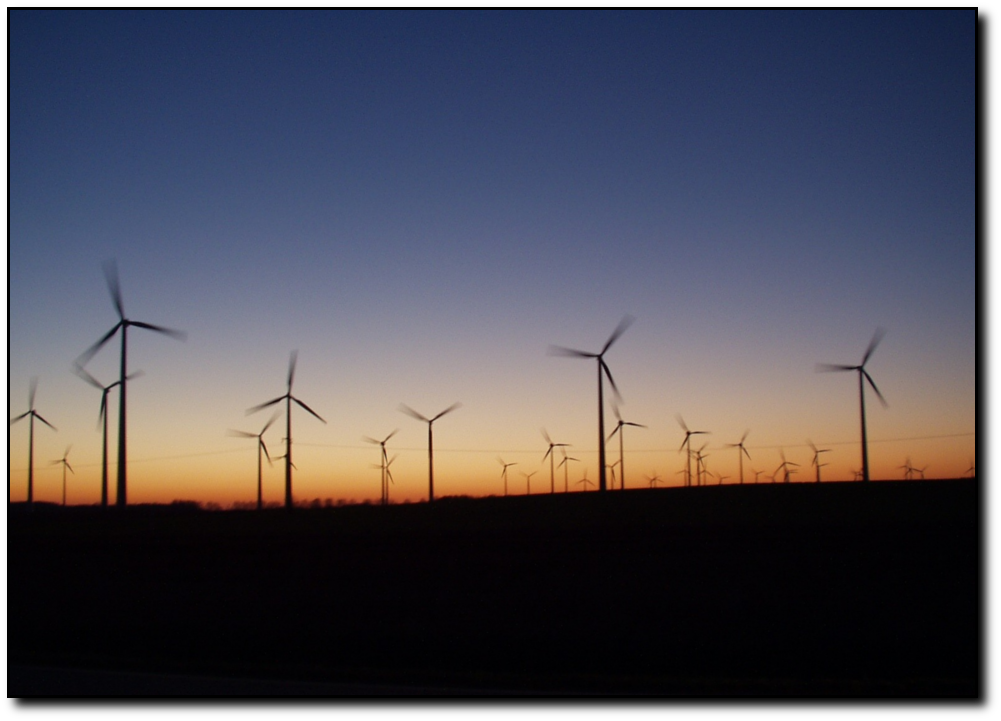
\includegraphics[width=1\textwidth]{pictures/deckblatt/Windpark.png}
  \caption{Windpark}
  \label{pic:Windpark}
\end{figure}

\newpage
%%%%%%%%%%%%%%%%%%%%%%%%%%
%%%%%%%%Neue Seite%%%%%%%%
%%%%%%%%%%%%%%%%%%%%%%%%%%

\section{Entstehung von Windenergie}


Die Hauptursache warum Winde entstehen, sind meist Unterschiede im Luftdruck
zwischen den Luftmassen. Hierbei gibt es \textsc{Hochdruckgebiete}\index{Hochdruckgebiete} (höherer Luftdruck)
und \textsc{Tiefdruckgebiete}\index{Tiefdruckgebiete} (geringerer Luftdruck). So lange bei diesen Gebieten ein
Luftdruckunterschied herrscht, wird versucht diesen Unterschied auszugleichen,
Winde entstehen. Je größer der Druckunterschied zwischen den beiden Gebieten
ist, desto stärker ist der Wind.\\

Es gibt jedoch auch natürliche Gegebenheiten, bei denen der Wind verstärkt wird. Eshandelt sich um unterschiedliche 
Effekte.

\subsection{Thermik-Effekte}
\index{Thermik-Effekte}

{\bfseries Seewind:} \\ \index{Seewind}
Er weht Tagsüber in Richtung Küste. Durch die Sonne wird das Land Tags mehr
erhitz als das Wasser. An Land steigt dann warme Luft auf, damit kein Vakuum
entsteht, wird durch das Meer kalte Luft hinzugeführt. Der Seewind fängt
mittags an und erreicht ca. 2 Stunden, nachdem die Sonne ihren höchsten Stand
hatte seinen Höhepunkt. Die Stärke des Seewindes hängt von der
Temperaturdifferenz zwischen Land und Wasser ab. Der Wind ist besonders am
Mittelmeer stark ausgeprägt, an den Küsten der Ostsee ist der See wind jedoch
auch recht stark und kann bis zu 5-10 km aufs Meer hinausreichen. Perfekte
Bedingungen für \textsc{Offshore-Parks}\index{Offshore-Parks} in der Nordsee.\\
\\
{\bfseries Landwind:}\\  \index{Landwind}
Er weht nachts in Richtung Meer. An Land kühlt sich die Luft nun 
schneller ab als über dem Meer, so kann über dem Meer eine warme 
Luft aufsteigen. Hier wird ein Vakuum über dem Meer durch ein Nachströmen 
kalter Luft vom Land unterstützt. Je höher die Temperaturdifferenzen zwischen Land 
und Wasser sind wird der Landwind stärker.\\



\subsection{Kap-Effekte}
\index{Kap-Effekte}

Treten überall da auf wo es Landnasen gibt (Kap, Huk) der Wind komm nun von
der Seite, am Scheitelpunkt des Kaps kommt es zu den heftigsten Winden,
unteranderem kann hier eine Verstärkung von 50\% stattfinden. Je mehr diese
Landnase aus einer Küstenlinie herausragt, desto stärker ist der Effekt. Auch
an diesen verstärkten Winden können Windkraftanlagen platziert werden.


\newpage
%%%%%%%%%%%%%%%%%%%%%%%%%%
%%%%%%%%Neue Seite%%%%%%%%
%%%%%%%%%%%%%%%%%%%%%%%%%%


\subsection{Düsen-Tunnel-Effekte}
\index{Düsen-Tunnel-Effekte}

{\bfseries Düsen-Effekt:}\\  \index{Düsen-Effekt}
Wenn der Wind durch zwei eng beieinander liegenden Landmassen weht, wird er
gestaucht, dadurch muss er mit hohen Geschwindigkeiten diesen Engpass mit
einer hohen Geschwindigkeit überwinden. Die Verstärkung des Windes Spürt man
bei der engsten Stelle und danach, der Wind kann sehr stark zunehmen. Der
Düseneffekt wird stärker, je höher die Landmassen beider Seiten sind.\\
\\
{\bfseries Tunnel-Effekt:}\\  \index{Tunnel-Effekt}
Er tritt im Tal auf. Er tritt dann auch zwischen eng aneinander liegenden
Landmassen auf, sonst ähnelt er dem Düsen-Effekt.

\subsection{Fallwind-Effekte}
\index{Fallwind-Effekte}

 Sie entstehen wenn ein Kaltluftpaket aus über 1000 m in ein Tal fällt. 
 
  \begin{wrapfigure}[7]{r}{0.51\textwidth}
 	\vspace{-20pt}
	\centering
    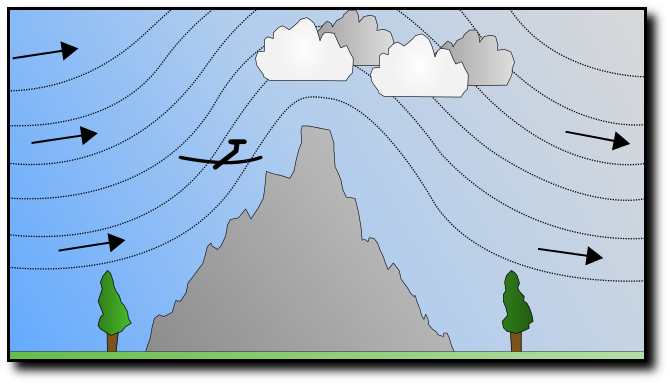
\includegraphics[width=0.50\textwidth]{pictures/adrian/Hangwind.png}
 % 	\vspace{-20pt}
  	\caption{Darstellung Fallwind}
  	\label{pic:Darstellung Fallwind}
\end{wrapfigure}
 Die dabei entstehen Windverstärkungen sind enorm. Es können \\
 Windgeschwindigkeiten  von bis zu 200 km/h entstehen. Für Winde im 
 Alpenraum wird die Bezeichnung Alpenföhn verwendet. 
 Auf der Abbildung: \ref{pic:Foehnwolken} werden Fallwinde im Alpenraum dagestellt.
 
 \vspace{1.6cm}
 \begin{figure}[htbp] 
  \centering
     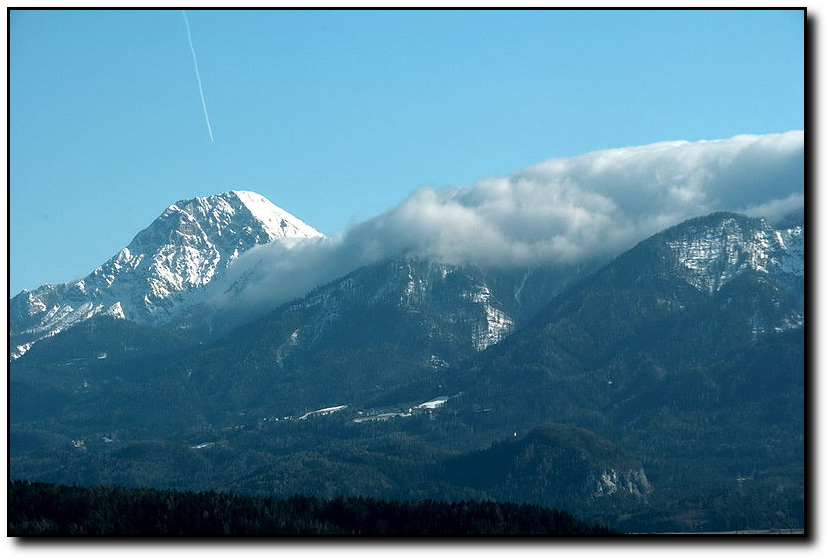
\includegraphics[width=0.9\textwidth]{pictures/adrian/Foehnwolken.png}
  \caption{Föhnwolken}
  \label{pic:Foehnwolken}
\end{figure}
 
 \newpage
%%%%%%%%%%%%%%%%%%%%%%%%%%
%%%%%%%%Neue Seite%%%%%%%%
%%%%%%%%%%%%%%%%%%%%%%%%%%

\section{Technik der Windkraftanlagen}


Die Windkraftanlagen setzen sich aus unterschiedlichen Komponenten zusammen. Diese werden in den folgenden 
Punkten beschrieben. 

\subsection{Rotorblätter}

 Mit den \textsc{Rotorblätter}\index{Rotorblätter} (Abbildung: \ref{pic:Fluegel einer Windkraftanlage}) wird die Windenergie der Luft entnommen und auf den
 Generator geleitet. Zudem sind sie für ein Teil des Betriebsgeräusches
 verantwortlich, deshalb werden sie nicht nur auf einen höheren Wirkungsgrad
 sondern auch auf eine Lärmreduzierung verbessert. 
 
 \begin{wrapfigure}[16]{r}{0.56\textwidth}
 	\vspace{-20pt}
	\centering
    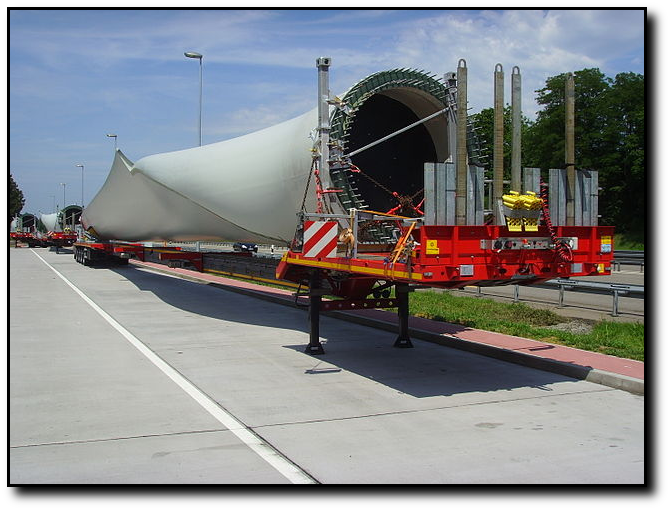
\includegraphics[width=0.55\textwidth]{pictures/adrian/Windkraftanlage_fluegel.png}
 % 	\vspace{-20pt}
  	\caption{Flügel einer Windkraftanlage}
  	\label{pic:Fluegel einer Windkraftanlage}
\end{wrapfigure}
 Bei den kleineren \\
 \textsc{Onshore-Windkraftanlagen}\index{Onshore-Windkraftanlagen} ist ein Rotordurchmesser von 60-90 m üblich, die
 größeren Anlagen können schon einen Rotordurchmesser von 120 - 130 m haben.
 Die Aktuellen \textsc{Offshore-Windräder}\index{Offshore-Windräder} verfügen über einen Durchmesser von ca. 90
 bis 126 m. Es sind jedoch Anlagen mit 170 m Durchmesser geplant. Moderne
 Rotorblätter von Windkraftanlagen bestehen aus glasfaserverstärkten
 Kunststoff. Vermehrt kommen bei großem Rotordurchmesser Rotorblätter aus \\
 Kohlenstofffasern fort. Zudem sind die Rotorblätter vor Blitzen gesichert,
 schlägt ein Blitz ein, wird der Blitz zur Erdung des Maschinenhauses
 geleitet.


\subsection{Maschinenhaus}

Das \textsc{Maschinenhaus}\index{Maschinenhaus} wird auch als Gondel bezeichnet und besteht aus dem
Triebstrang, der elektrischen Ausrüstung, der Windrichtungsnachführung,  der
Rotorkopflagerung sowie Hilfsfausrüstung wie z.B. Kühlsysteme, Elektronik usw.
Obwohl das Maschinenhaus im Vergleich zu anderen Techniken schwierig zu
montieren ist. Ein Vorteil des hoch liegenden Maschinenhauses sind die kurzen
Übertragungswege. Im Maschinenhaus befinden sich auch eine Heizung,
Feuerlöscher, die Öl- und Hydraulikversorgung und Datenerfassung. In an
manchen Maschinenhäusern befinden sich auch Kräne, mit diesen können größere
Komponenten der Anlage nach oben befördert und montiert werden ohne einen
mobilen Kran zu rufen. Auf den Offshore-Anlagen befindet sich zudem meist noch
ein Helikopterlandeplatz.

\newpage
%%%%%%%%%%%%%%%%%%%%%%%%%%
%%%%%%%%Neue Seite%%%%%%%%
%%%%%%%%%%%%%%%%%%%%%%%%%%


\subsection{Nabe}

Die \textsc{Nabe}\index{Nabe} (Abbildung: \ref{pic:Nabe}) wird zwar oft als Teil des Rotors gesehen, sie stellt jedoch die
erste mechanische Komponente dar. 

\begin{wrapfigure}[12]{r}{0.31\textwidth}
	\vspace{-10pt}
	\centering
    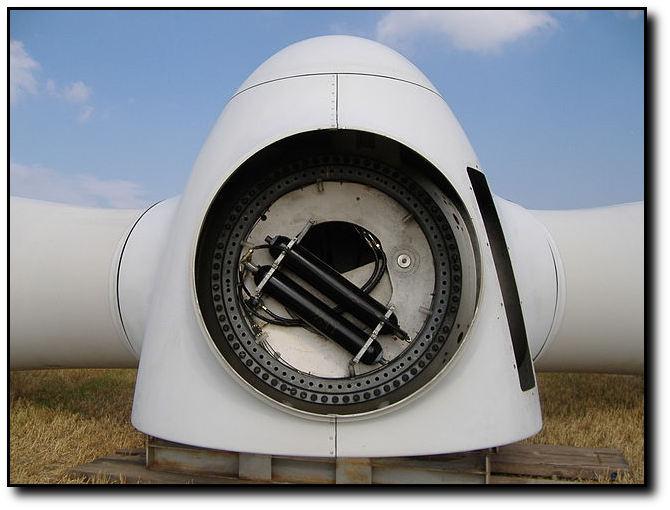
\includegraphics[width=0.30\textwidth]{pictures/adrian/Rotorblatt_Achse.png}
 % 	\vspace{-20pt}
  	\caption{Nabe}
  	\label{pic:Nabe}
\end{wrapfigure}
Hier sind die Komponenten zur Blatteinstellung untergebracht, zur Blatteinstellung wir meist ein
hydraulischer, aber auch ein elektrischer Motor eingesetzt. In der Nabe ist
jedoch auch eine Notstromversorgung, mit ihr kann sich die Anlage sicher
abschalten und Bremsen, falls es zu einer Netzunterbrechung kommen sollte. Da
die Nabe eines der meist belastet Teile der Windkraftanlage sind, wird bei
ihrer Fertigung besonders Acht gegeben. Die Naben moderner Windkraftanalgen
bestehen sowohl aus Stahlguss, als auch aus speziellen Kugelgraphitguss.



\subsection{Getriebe}

Das \textsc{Getriebe}\index{Getriebe} der Windkraftanlage hat die Aufgabe die langsamen Umdrehungen der
Rotoren auf den schnelllaufenden Generator zu übertragen. Am Anfang der
Windenergienutzung, wurden die Getriebe meist falsch dimensioniert oder
mangelhaft gebaut, doch im Laufe der Jahre hat man das Getriebe perfekt auf
seine Aufgabe angepasst. Als Bauformen kommen die \textsc{Planetengetriebe}\index{Planetengetriebe}, sowie
Stirnradgetriebe vor.

\subsection{Bremse}

Die \textsc{Bremse}\index{Bremse} ist eine Sicherung für den Notfall. Sie muss dann die komplette
Bewegungsenergie der Rotoren und des Generators aufnehmen können. Deshalb muss
die Bremse sehr leistungsfähig sein. Sie werden aber auch als Betriebsbremsen
benutz, um den Rotor bei Windböen innerhalb der Toleranz zu halten. In den
Windrädern sind meist Scheibenbremsen verbaut. Jede Anlage muss aber zwei
voneinander unabhängige Bremssysteme haben, dazu zählen aber auch die Rotoren,
die sich unabhängig voneinander einstellen können muss.


\subsection{Generator}

Der \textsc{Generator}\index{Generator} wird für eine Umwandlung von mechanischer in elektrischer
Energie benötigt, es wird entweder ein Asynchroner- oder ein Synchroner-
Generator verwendet. Im Laufe der Jahre wurde der Generator auf mehr auf
Leistung, Kosten und Gewicht verbessert. Die Drehzahl des Generators kann
heutzutage auf konstant, zweistufig oder stufenlos eingestellt werden.


\subsection{Windrichtungsnachführung}

Bei modernen Windkraftanlagen erfolgt die \textsc{Windrichtungsnachführung}\index{Windrichtungsnachführung} durch
Stellmotoren. Die Windrichtung wird erst durch Sensoren, den so genannten
\textsc{Windrichtungsgebern}\index{Windrichtungsgebern} festgelegt. Die elektrischen Verbindungen bestehen aus
festen Kabeln und nicht aus Schleifkontakten weil diesem bei den hohen Strömen
zu uneffektiv sind. Dank der Windnachrichtungsführung kann man die Leistung
der Windkraftanlagen enorm verstärken und somit den Wirkungsgrad erhöhen.


\newpage
%%%%%%%%%%%%%%%%%%%%%%%%%%
%%%%%%%%Neue Seite%%%%%%%%
%%%%%%%%%%%%%%%%%%%%%%%%%%

\subsection{Turm}

Der \textsc{Turm}\index{Turm} der Windkraftanlage muss sehr stabil sein, da er besonders hohen
Belastungen standhalten muss. So können Gondel und Roter ein Gewicht von
mehreren hundert Tonnen haben. Ein weiteres Problem ist jedoch der Wind, der
mit hoher Kraft gegen den Turm drückt. Je höher der Turm desto mehr Kraft muss
der Turm vor allem am Fundament aushalten. Bei der Konstruktion muss zudem
noch bedacht werden, dass der riesige Turm  zu seinem späteren Standort
transportiert werden muss. Die Turmhöhe variiert je nach Standort. An
Küstenstandorten werden kleiner Türme wegen der See und Landwinde verwendet,
man hat jedoch errechnet, das im Binnenland pro zusätzlicher Meter Höhe 0,8\%
mehr Strom erzeugen kann. 2010 wurden am häufigsten die Türme gebaut, die eine
Nabenhöhe von 100 oder 120 Meter haben, diese Gruppe macht auch 34,4\% der
installierten Türme in Deutschland aus. Die 81 - 100 Meter hohen Türme machen
20\% und 61 - 80 24,7\% aus. Den kleinsten Teil machen die Windräder aus, die
kleiner als 60m sind (4,2\%). Trotzdem haben schon 16,6\% der Anlagen eine
Nabenhöhe höher als 120 Meter. Die meisten Türme bestehen aus Stahl und werden
in großen Stücken an die Baustelle geliefert. Hierbei besteht ein Turm aus
durchschnittlich aus zwei bis vier Teilen, die Wandstärken betragen hier
zwischen 20 bis 60 Millimeter. Bei sehr großen Türmen wird der unterste Teil
des Turms aus Beton gefertigt. Es gibt aber auch Türme, die aus Gittermästen
gefertigt sind. Eine komplett neue Idee ist der Turmbau aus Holz. Hierbei wird
eine geschlossene Holzröhre verwendet. Diese Technik soll noch
Umweltverträglicher sein, aber trotzdem noch stabil genug um den enormen
Kräften stand zu halten. Es gibt bereits einen Prototyp, der in Hannover
errichtet wurde.

\subsection{Fundament}
\index{Fundament}


Eine Windkraftanlage muss fest im Boden verankert sein. Bei den Fundamenten
werden Flachgründungsfundamente benutz, diese sind sehr stabil, verbrauchen
jedoch viel Platz. Eine andere Möglichkeit sind die Pfahlfundamente, diese
brauchen weniger Platz, halten aber trotzdem die hohen Zugkräfte der
Windkraftanlage aus. Bei Offshoreanlagen werden jedoch andere Fundamente
benutz, hier kommen Tripod-, Bucket- und Pfostenfundamente benutzt.\\
\textsc{Tripod-Fundamente}\index{Tripod-Fundament} sind wie ein Dreifuß auf gebaut. \\
Das \textsc{Bucket-Fundament}\index{Bucket-Fundament} ist wie ein Zylinder (Bucket ist das englische Wort für Eimer) der auf den
Meeresgrund gelassen wird, hier wird er dann leergepumpt und so saugt er sich
aufgrund des entstandenes Unterdrucks am Meeresgrund fest. \\
Beim \textsc{Pfostenfundament}\index{Pfostenfundament} wird einfach ein zusätzlich langer Pfosten am Meeresgrund
angebracht. \\
Eine neue Entwicklung ist die schwimmende Windkraftanlage, hier
wird die Windkraftanalge auf einen riesigen Schwimmkörper gebaut, so ist sie
Mobil und man kann an den tiefsten Stellen Windenergie in elektrische Energie
umwandeln.



\newpage
%%%%%%%%%%%%%%%%%%%%%%%%%%
%%%%%%%%Neue Seite%%%%%%%%
%%%%%%%%%%%%%%%%%%%%%%%%%%

\subsection{Darstellung einer Windkraftanlage}


\begin{figure}[htbp] 
  \centering
     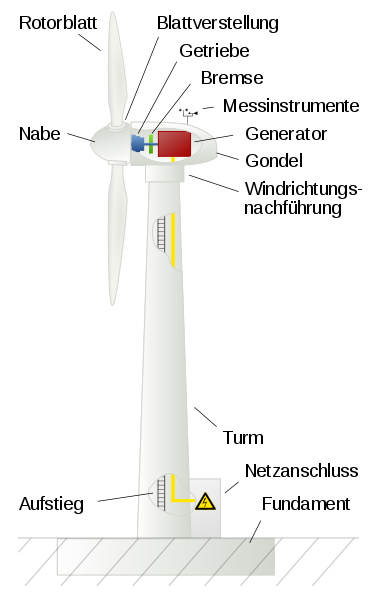
\includegraphics[width=0.7\textwidth]{pictures/adrian/windkraftanlage.png}
  \caption{Aufbau einer Windkraftanlage}
  \label{pic:Windkraftanlage}
\end{figure}




\newpage
%%%%%%%%%%%%%%%%%%%%%%%%%%
%%%%%%%%Neue Seite%%%%%%%%
%%%%%%%%%%%%%%%%%%%%%%%%%%


\section{Wirtschaftlichkeit}
\index{Wirtschaftlichkeit}

Wie in (Abbildung \ref{pic:Historische Anlage}) dargestellt, gab es vor über 100 
Jahre Windkraftanlagen. Die darstellte Anlage stammt aus dem Jahr 1880.\\
Die Zukunftssicherheit der Windkraftanlagen ist sehr gut, da Windkraft überall
und immer verfügbar ist, so fällt bei Windkraft die Autarkie aus, das heißt
jedes Land kann Windkraft nutzen. Ein gutes Beispiel für ein Gegenteil wäre
Russland oder Arabien. Hier ist ein Überfluss an Öl und anderen wertvollen
Bodenschätzen vorhanden, während in Deutschland solche Quellen nicht vorhanden
sind. Zudem ist Wind unerschöpflich und kann nicht versiegen (wie z.B. eine
Ölquelle). 

 \begin{wrapfigure}[28]{r}{0.56\textwidth}
 	\vspace{-10pt}
	\centering
    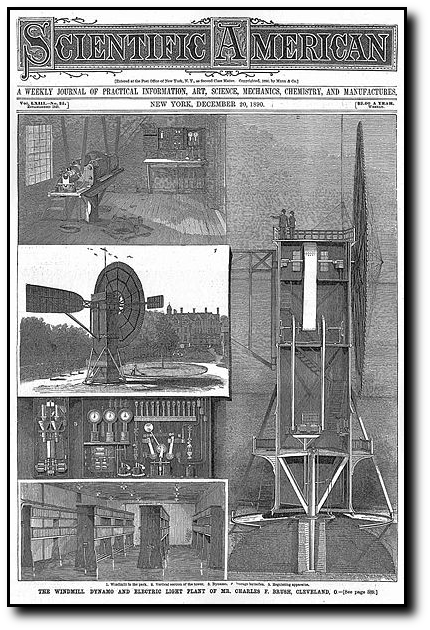
\includegraphics[width=0.55\textwidth]{pictures/adrian/historisch_windmill.png}
 % 	\vspace{-20pt}
  	\caption{Historische Anlage}
  	\label{pic:Historische Anlage}
\end{wrapfigure}
Trotzdem kostet eine Windkraftanlage Geld, die Kosten variieren je
nach Nennleistung. Eine große Windkraftanlage  hat eine Nennleistung von 1-2,5
Megawatt. Der Strom einer Windkraftanlage kann bis zu 1000 Euro pro Kw kosten,
bei einer großen Windkraftanlage macht das dann bis zu 2,5 Mio. Euro. Das
teuerste an der Windkraftanlage ist der Turm und der Rotor, sie machen fast
die Hälfte der Anlagenlosten aus. Weitere teure Teile sind das Getriebe und
der Generator. Zu den Anlagenkosten, die ca. 70-80\% der \textsc{Anfangsinvestitionen}\index{Anfangsinvestitionen}
ausmachen kommen die \textsc{Investitionsnebenkosten}\index{Investitionsnebenkosten}. Hier sind das Fundament und die
Netzanbindung das Hauptproblem. Damit ist es jedoch nicht getan. Bei
Windkraftanlagen fallen genauso die Wartungskosten an, die ebenfalls einen
großen Teil des Investitionsgeldes\footnote{Geld zur Finanzierung der Windkraftanlagen} verschlingen. Zudem muss auch eine
Windkraftanlage versichert sein, auch eine Pacht muss meistens bezahlt werden.
Die Betriebs- und Wartungskosten steigen mit dem Alter der Anlage. Moderne
Windkraftanlagen sind heute darauf ausgelegt 20 Jahre Strom zu produzieren.

\newpage
%%%%%%%%%%%%%%%%%%%%%%%%%%
%%%%%%%%Neue Seite%%%%%%%%
%%%%%%%%%%%%%%%%%%%%%%%%%%


\section{Auswirkung auf die Umwelt}
\index{Windkraftanlage Auswirkung Umwelt}

Doch auch die Windkraftanlage hat Nachteile beim Thema Umwelt. Die am meisten
bedrohten Tiere durch Windkraftanlagen sind die Vögel und Fledermäuse. Viele Tiere (Abbildung: \ref{pic:Verletzter Seeadler})
werden bei einen Zusammenstoß mit einer Windkraftanlage schwer verletzt. 

\begin{wrapfigure}[19]{r}{0.61\textwidth}
 	\vspace{-20pt}
	\centering
    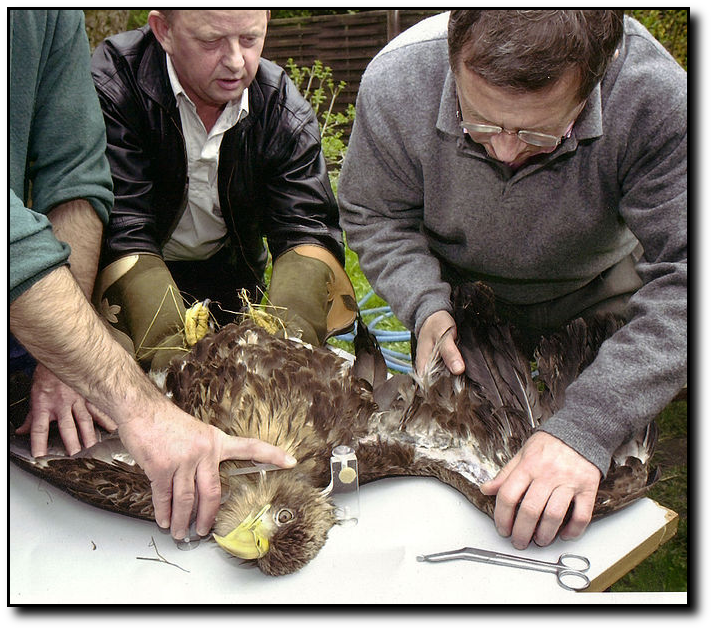
\includegraphics[width=0.60\textwidth]{pictures/adrian/Seeadler_und_Windrad.png}
 % 	\vspace{-20pt}
  	\caption{Verletzter Seeadler}
  	\label{pic:Verletzter Seeadler}
\end{wrapfigure}
Jährlich sterben etwa 0,5 Tiere pro Windkraftanlage. 2005 existierten bereits
2000 Anlagen in Deutschland, das machte 1000 getötete Tiere allein im Jahr
2005. Zudem bedrohen manche Windkraftanlagen die Wanderrouten der Vögel, die
entweder in Richtung Süden oder zurück nach Deutschland möchten. Auch viele
Fledermäuse verunglücken nachts, \\
wenn sie auf Beutezug sind. Auch die kleinen
wendigen Fledermäuse sind vor den schnell drehenden Rotoren nicht sicher. Um
diese Tiere zu schützen, haben Umweltschützer beschlossen, \\
einzelne Windanlagen abzubauen und dafür leistungsstärkere Parks zu installieren, genau
da, wo weniger der bedrohten Tiere vertreten sind.


\newpage
%%%%%%%%%%%%%%%%%%%%%%%%%%
%%%%%%%%Neue Seite%%%%%%%%
%%%%%%%%%%%%%%%%%%%%%%%%%%


\section{Auswirkung auf die Gesellschaft}
\index{Windkraftanlage Auswirkung Gesellschaft}

Eine Umfrage aus dem Jahr 2009 hat ergeben, dass die Gesellschaftliche
Akzeptanz von Windkraftanlagen in der eigenen Nachbarschaft relativ hoch ist:
Zudem ist die Akzeptanz besonders hoch, wenn man Erfahrung mit
Windkraftanlagen gesammelt hat. So liegt die Zustimmung von Windkraftanlagen
bei der Gesamtbevölkerung von 55\%. Bei Personen, die bereits eine
Windkraftanlage in der Nachbarschaft haben sogar bei 75\%. Zudem steigt die
Bereitschaft für Windkraftanlagen stetig an, vor allem bei Umfragen nach dem
Fukushima Unglück waren immer mehr Leute bereit auf Atomkraft zu verzichten.
Es gibt jedoch auch Bürger die Windkraftanlagen ablehnen. Hier haben sich
sogar Bürgerinitiativen gegründet die gegen Windkraftanlagen in ihrer näheren
Umgebung sind. Es gibt jedoch auch gesellschaftliche Probleme, die bei
Windkraftanlagen auftreten.


\subsection{Schattenwurf}


Der \textsc{Schattenwurf}\index{Schattenwurf} einer Windkraftanlage kann sehr störend sein. Aufgrund der
sich ständig drehenden Rotoren entsteht eine permanente Helligkeitsschwankung.
Laut dem Bundesemissionsgesetz darf der Schatten eines Windrades nur 30
Minuten am Tag oder 30 Stunden pro Jahr auf ein Wohngebäude fallen.


\subsection{Disko-Effekt}

Beim \textsc{Disko-Effekt}\index{Disko-Effekt} wird von den Rotoren der Windräder die Sonne reflektiert und
kann dadurch blenden wirken. Der Diskoeffekt trat vor bei den Anlagen, die zum
Anfang der Windenergienutzung benutzt wurden auf. Auf ihren Rotoren befand
sich ein glänzender Lack. Bei den neusten Anlagen wird jedoch ein matter Lack
benutzt, hier fällt der Disko-Effekt dann aus.

\subsection{Hindernis-Befeuerung}
\index{Hindernis-Befeuerung}

Da die meisten Windkraftanlagen 100 Meter oder höher sind, sind sie leicht
Hindernisse für den Flugverkehr. Damit es nicht zum Crash kommt, haben deshalb
alle Windkraftanlagen Leuchtstoffröhren, bei den neueren Anlagen LED's als
Signalleuchten. So könne sie (vor allem bei größeren Ansammlungen) störend auf
die Anwohner wirken. Doch eine Lösung ist schon in Sicht, es werden spezielle
Radarsysteme entwickelt, bei denen die Windkraftanlage frühzeitig erkennt,
wenn ein Flugzeug in die Nähe kommt und sich erst dann einschaltet.


\subsection{Schall}

Eine Windkraftanlage kann einen \textsc{Schall}\index{Schall} von 98 - 109 und mehr dB erzeugen.
Dieser Schallpegel wird jedoch direkt am Windrad gemessen, wenn die
Windkraftanlagen eine angemessene Entfernung zur Wohnsiedlung hat, kann man
eine Windkraftanlage nur bei einer Windgeschwindigkeit von 10m/s deutlich
hören. So ist der Schalleinfluss einer Windkraftanlage liegt bei einer 500
Meter entfernen Wohnsiedlung nur noch bei 45 dB. Es gibt auch Drehzahlvariable
Windräder, hier kann dann z.B. wenn es Nacht ist die Windkraftanlagen
langsamer drehen lassen, so werden sie leiser und stören niemanden.


\newpage
%%%%%%%%%%%%%%%%%%%%%%%%%%
%%%%%%%%Neue Seite%%%%%%%%
%%%%%%%%%%%%%%%%%%%%%%%%%%

\subsection{Infraschall}

Bisher (2013) konnte ein gesundheitlicher Einfluss von Windkraftanlagen
erzeugten \textsc{Infraschall}\index{Infraschall} nicht nachgewiesen werden. In der Umgebung einer
Windkraftanlage liegt Infraschallanteile deutlich unter der menschlichen
Wahrnehmung.  So liegt der Schallpegel von Tieffrequenten Geräuschen in einem
Schnellfahrenden Auto bei 8 - 100 Hertz, zum Vergleich, eine Windkraftanlage
erzeugt bei einer Windgeschindigkeit von 6m/s in einer Entfernung von 250
Meter eindeutig weniger. So liegen die tieffrequenten Töne bei der
Windkraftanlage "`nur"' bei 40 Hertz, bei einem Auto ja deutlich unter 20 Herz.
Es gibt Fälle von Gesundheitlichen Problemen in der Nähe von Windkraftanlagen,
eine Studie hat jedoch belegt, dass diese Beschwerden nicht aufgrund des
Infraschalls sondern aufgrund vor der Angst des Infraschalls sind. Dies wurde
bei einem Test bewiesen, als man mit zwei Gruppen von Testpersonen zwei
unterschiedliche Situationen nachstellte, die einen bekamen erklärt, das
Infraschall nicht schädlich ist und den anderen wurde erzählt das man sie den
"`gefährlichen"' Infrastrahlen aussetzen würden, zudem erklärte man ihnen
bestimmte Symptome. Den richtig Informierten passierte nichts, doch bei den
falsch informierten traten die vorher erklärten Symptome auf. Wissenschaftler
nenne es den Nocebo-Effekt.

\subsection{Einfluss auf Radaranlagen}

Da Windräder die Reichweite von \textsc{Radaranlagen}\index{Radaranlagen} mindern, gibt es für Windräder die
in der Nähe von Radargeräten gebaut werden Baueinschränkungen. Durch die
drehenden Rotoren erhält das Radarecho ein Helikopter ähnliches Aussehen. So
kann es zum Beispiel zu einem Fehlalarm kommen.

\subsection{Immobilienpreise}

Eines der meisten benutzen Argumente von den Bürgerinitiativen sind die
dauerhaft sinkenden \textsc{Immobilienpreise}\index{Immobilienpreise}, die in der Nähe von Windkraftanalgen
sinken. Laut Phillip Thalman löst die Angst vor dem Preisrückgang den
eigentlichen Preisrückgang auslösen. So kommt es gerade da zum großen
Preisrückgang der Immobilien wo es einen großen Wiederstand gegen die
Windkraftanlagen gibt. Die Einbrüche der Immobilienpreise sind wohl nur so
lange ein Problem, bis sich die Bewohner an die Windräder gewöhnt haben.

\subsection{Tourismus}
\index{Tourismus}

Vor allem in Regionen, die touristisch bedeutsam sind, wird ein Rückgang der
Übernachtungszahlen befürchtet, dies ist bis jetzt jedoch noch nicht bewiesen.
Selbst nach einer Umfrage an Touristen fand nur eine kleine Gruppe an
Urlaubern die Windräder als störend. Die meisten Urlauber die gegen die
Windräder waren, waren entweder alte Menschen oder überhaupt gegen
Windenergie.

\newpage
%%%%%%%%%%%%%%%%%%%%%%%%%%
%%%%%%%%Neue Seite%%%%%%%%
%%%%%%%%%%%%%%%%%%%%%%%%%%

\chapter{Solarzelle und Photovoltaik (Stefan Nuber)}

\begin{figure}[htbp] 
  \centering
     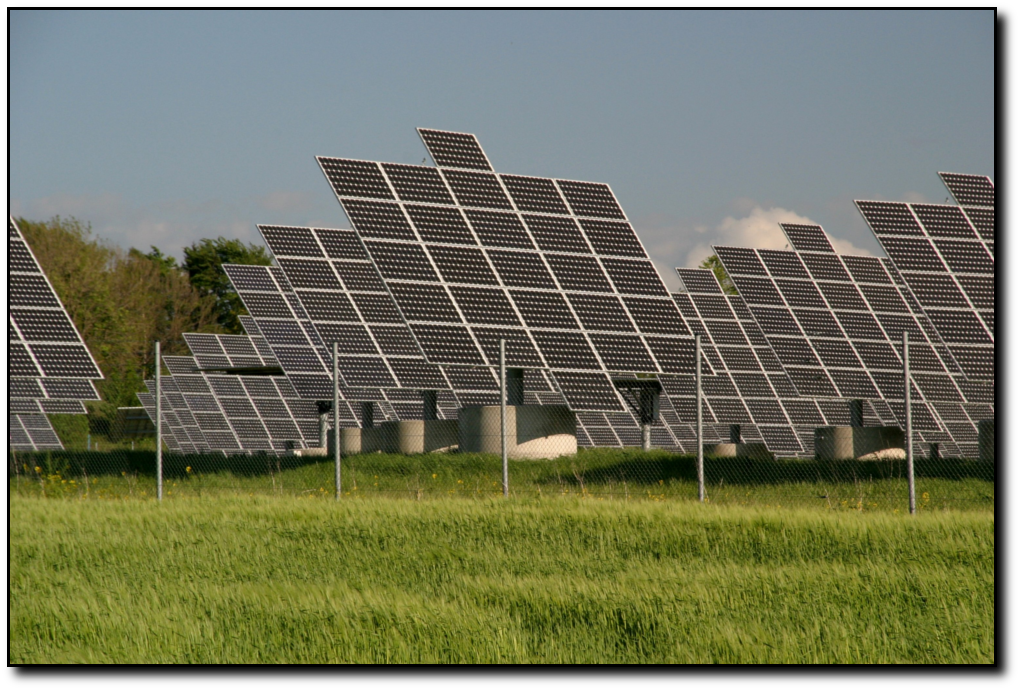
\includegraphics[width=1\textwidth]{pictures/deckblatt/Solaranlage_IMG_0533.png}
  \caption{Photovoltaikanlage}
  \label{pic:Photovoltaikanlage}
\end{figure}


\newpage
%%%%%%%%%%%%%%%%%%%%%%%%%%
%%%%%%%%Neue Seite%%%%%%%%
%%%%%%%%%%%%%%%%%%%%%%%%%%

\section{Aufbau einer Solarzelle}

\textsc{Solarzellen}\index{Aufbau einer Solarzelle} bestehen in der Regel aus dem Halbleitermaterial Silizium. Der
Grund dafür ist, dass \textsc{Halbleitermaterialien}\index{Halbleitermaterialien} bei zugeführter Energie, in diesem
Fall die Sonnenstrahlung, freie Ladungsträger erzeugen. Der eigentliche Aufbau
ist aber, dass eine Solarzelle zwei Schichten hat. Zum einen eine n-Dotierte
Schicht (in der sich die Elektronen befinden) und eine p-Dotierte Schicht (in
der sich die Protonen befinden). Um dass aber Vollständig zu verstehen, muss
man wissen was eine Dotierung ist. Eine \textsc{Dotierung}\index{Dotierung} ist eine gezielte
Verunreinigung mit Fremdatomen, die das Ausgangsmaterial leitfähiger oder
weniger leitfähig machen. Man spricht von p- und n-Dotierung. Bei der
p-Dotierung sind weniger freie Elektronen vorhanden und bei der n-Dotierung
sind mehr freie Elektronen vorhanden. In diesem Fall wird alles logisch. Um
sich den Aufbau einer Solarzelle schließlich vorstellen zu können muss man
sich Abbildung \ref{pic:Aufbau Solarzelle} betrachten. Hier sieht man zusätzlich den Kontaktfinger, die
Antireflexschicht, den Verbraucher und den Metallkontakt. Diese sind aber zu
vernachlässigen. Wichtig sind die n-Halbleiterschicht, der p/n-Übergang und
die p-Halbleiterschicht.



\begin{figure}[htbp] 
  \centering
     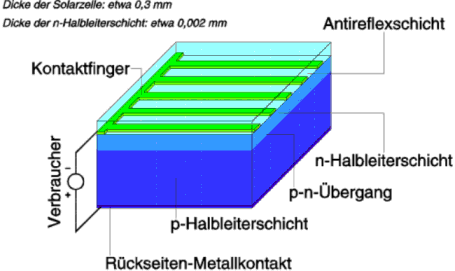
\includegraphics[width=1\textwidth]{pictures/stefan/stefan_001.png}
  \caption{Aufbau einer Solarzelle}
  \label{pic:Aufbau Solarzelle}
\end{figure}

\newpage
%%%%%%%%%%%%%%%%%%%%%%%%%%
%%%%%%%%Neue Seite%%%%%%%%
%%%%%%%%%%%%%%%%%%%%%%%%%%


\section{Funktion einer Solarzelle}

Man kann die Funktion einer \textsc{Solarzelle}\index{Funktion einer Solarzelle} mit einem übertragenem Wassermodell
beschreiben. Wenn man sich vorstellt, dass in einer Solarzelle zwei Ebenen in
unterschiedlichen Höhen verbaut sind und in der unteren Ebene befinden sich
Löcher gefüllt mit Wasser, die obere Ebene ist dagegen glatt. Wenn man jetzt
etwas in die Löcher wirft spritzt das Wasser auf die obere Ebene. Diese Ebene
ist leicht geneigt, sodass das Wasser abfließt und einen Dynamo, der den
elektrischen Strom erzeugt, antreibt. Dann fließt dass Wasser wieder auf die
untere Ebene in die Löcher. So oder so ähnlich läuft es mit dem elektrischen
Strom bzw. mit den Protonen und Elektronen. Man muss lediglich das Wasser
durch Elektronen ersetzten. Die Elektronen sind in der unteren Ebene oder der
p-Halbleiterschicht nicht frei beweglich. Trifft nun die Sonnenstrahlung auf
die p-Halbleiterschicht, so werden die Elektronen auf die n-Halbleiterschicht
angehoben. Die Lichtteilchen werden auch Photonen genannt. Durch ein
elektrisches Feld, der Raumladungszone (zwischen den Halbleiterschichten)
werden die Elektronen auf der zweiten Ebene auf eine Seite gebracht. Dafür
muss der Halbleiter zuerst dotiert werden. Über einen äußeren Stromkreis
gelangen die Elektronen auf die p-Halbleiterschicht zurück.


\begin{figure}[htbp] 
  \centering
     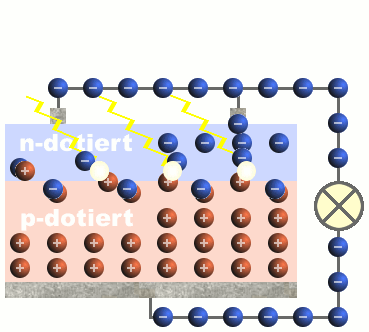
\includegraphics[width=1\textwidth]{pictures/stefan/stefan_002.png}
  \caption{Funktion einer Solarzelle}
  \label{pic:Funktion Solarzelle}
\end{figure}


\newpage
%%%%%%%%%%%%%%%%%%%%%%%%%%
%%%%%%%%Neue Seite%%%%%%%%
%%%%%%%%%%%%%%%%%%%%%%%%%%

\section{Typen von Siliziumzellen}
\index{Typen von Siliziumzellen}

In der Regel werden die Solarzellen aus dem Halbleitermaterial Silizium
hergestellt. Da es unterschiedliche Arten von Silizium gibt (Einkristalline
Siliziumscheiben oder nichtkristalline Siliziumscheiben), gibt es auch
unterschiedliche Arten von Siliziumzellen. Die am häufigsten Siliziumzellen sind:
\begin{itemize}
  \item Monokristalline Zellen
  \item Polykristalline Zellen
  \item Amorphe Solarzellen
  \item Mikrokristalline Zellen
  \item Tandem-Solarzellen
\end{itemize}

\section{Wirkungsgrad}

Der \textsc{Wirkungsgrad}\index{Wirkungsgrad einer Solarzelle} $\eta$ einer Solarzelle ist das Verhältnis der von ihr erzeugten 
elektrischen Leistung {\bfseries P elektrisch} und der Leistung der einfallenden Strahlung {\bfseries P Licht}.

\vspace{12pt}
\begin{LARGE}
\begin{math} \eta = \frac{P\ elektrisch}{P\ Licht} \end{math}
\end{LARGE}

\vspace{12pt}
Natürlich will man einen Höchstmöglichen Wirkungsgrad erzielen, da man bei
einem höheren Wirkungsgrad bei gleichen Lichtverhältnissen mehr elektrische
Energie erzeugen kann als bei einem geringen Wirkungsgrad.


\section{Umweltschutz}

Es wird oft behauptet, dass alles, was mit Regenerativen Energien zu tun hat
gleichzeitig die Umwelt schont und deshalb auch zum \textsc{Umweltschutz}\index{Umweltschutz} beiträgt, so
nach dem Motto es ist alles Gold was glänzt. Doch so wie eben nicht alles Gold
ist, was glänzt so sind die regenerativen Energien nicht immer Umweltschonend.

\section{Kohlendioxidbilanz}
\index{Kohlendioxidbilanz}

Ist die Solarzelle bzw. die Photovoltaikanlage erstmals in Betrieb, so bildet
sie keinen Kohlenstoffdioxid mehr, doch bis sie erstmals in Betrieb genommen
werden kann muss sie hergestellt werden und in der Produktion wird
Kohlenstoffdioxid freigesetzt. Der Prozess bei dem am meisten
Kohlenstoffdioxid entsteht, ist die Gewinnung des Silizium, dem Rohmaterial
der Solarzellen. Dennoch ist der Ausstoß des Kohlenstoffdioxids bei
Solarzellen nichts im Gegensatz zu den Kohlenstoffdioxid Ausstößen eines
Kohlekraftwerks ( 50-100 g/kWh bei einer Solarzelle und 750-1200 g/kWh bei
einem Kohlekraftwerk). Doch die Stromerzeugung durch die anderen
Regenerativen Energien Wind und Wasserkraft geht mit weniger CO2 Emissionen
von statten (10-40 g/kWh).

\section{Flächenverbrauch}

Photovoltaikanlagen führen dahingehen zu keinem weiteren \textsc{Flächenverbrauch}\index{Flächenverbrauch}, da
sie problemlos auf Dachflächen und Verkehrsflächen montiert werden können.
Zudem werden sie auch entlang von Autobahnen und Bahnlinien montiert, es
keinen Menschen stört. Sie werden aber auch auf Flächen, die als Industrie-
oder Gewerbeflächen ausgewiesen sind wie z.B. Deponien, Parkplätze etc.
gebaut. Zudem machen sie im Gegensatz zu Windrädern keinen Lärm.


\newpage
%%%%%%%%%%%%%%%%%%%%%%%%%%
%%%%%%%%Neue Seite%%%%%%%%
%%%%%%%%%%%%%%%%%%%%%%%%%%

\section{Wirtschaftlichkeit}

\subsection{Einspeisevergütung}

Seit dem Jahr 2011 sind die Stromgestehungskosten niedriger als der
Haushaltsstrompreis, was die Wirtschaftlichkeit unattraktiver gemacht hat.\\
\\
Grund dafür war, dass Menschen mit Photovoltaikanlagen ihren gesamten
produzierten Strom ins Stromnetz einspeisten und den billigeren Haushaltsstrom
von ihren Stromanbietern selber verbrauchten. Im Endeffekt heißt das, dass sie
mehr Geld für den Strom, den sie ins Stromnetz eingespeist haben, bekommen,
als sie für den normalen Haushaltsstrom ausgeben. Deshalb kostet jetzt der
Haushalsstrom mehr bzw. das Geld das man für die Einspeisung ins Netz bekommt
ist nicht mehr so hoch.

\subsection{Anschaffungskosten}

Die Anschaffungskosten einer Photovoltaikanlage sind je nach Typ und Größe
unterschiedlich. In der Regel benötigt man für eine Kilowattstunde 8 - 9 m$^2$
Fläche. Der Durchschnittliche Preis im Januar 2013 lag bei 1520\texteuro~Netto pro kW.
Der Preis setzt sich aber nicht nur aus den Modulen der Anlage zusammen,
sondern es setzt sich aus den Modulen, dem Wechselrichter, der Montage und dem
Netzanschluss zusammen. Doch mit der zeit können sich die Anschaffungskosten
vermindern, indem man den produzierten Strom oder einen Teil des produzierten
Stroms ins Netz einspeist.


\newpage
%%%%%%%%%%%%%%%%%%%%%%%%%%
%%%%%%%%Neue Seite%%%%%%%%
%%%%%%%%%%%%%%%%%%%%%%%%%%

\chapter{Quellenverzeichnis}

Bilder Deckblatt: \\
\url{http://de.wikipedia.org/wiki/Erneuerbare_Energie}\\

Bilder Titelseiten aller Kapitel: \\
\url{http://de.wikipedia.org/wiki/Erneuerbare_Energie}\\

Bilder Kapitel Windkraft (Adrian Imme):\\
\url{http://de.wikipedia.org/wiki/Windenergieanlage}\\
\url{http://de.wikipedia.org/wiki/F\%C3\%B6hn}\\

Bilder Sachregister: \\
\url{http://de.wikipedia.org/wiki/Erneuerbare_Energie}\\


\newpage
%%%%%%%%%%%%%%%%%%%%%%%%%%
%%%%%%%%Neue Seite%%%%%%%%
%%%%%%%%%%%%%%%%%%%%%%%%%%

\chapter{Index (Sachregister von A bis Z)}

\begin{center}
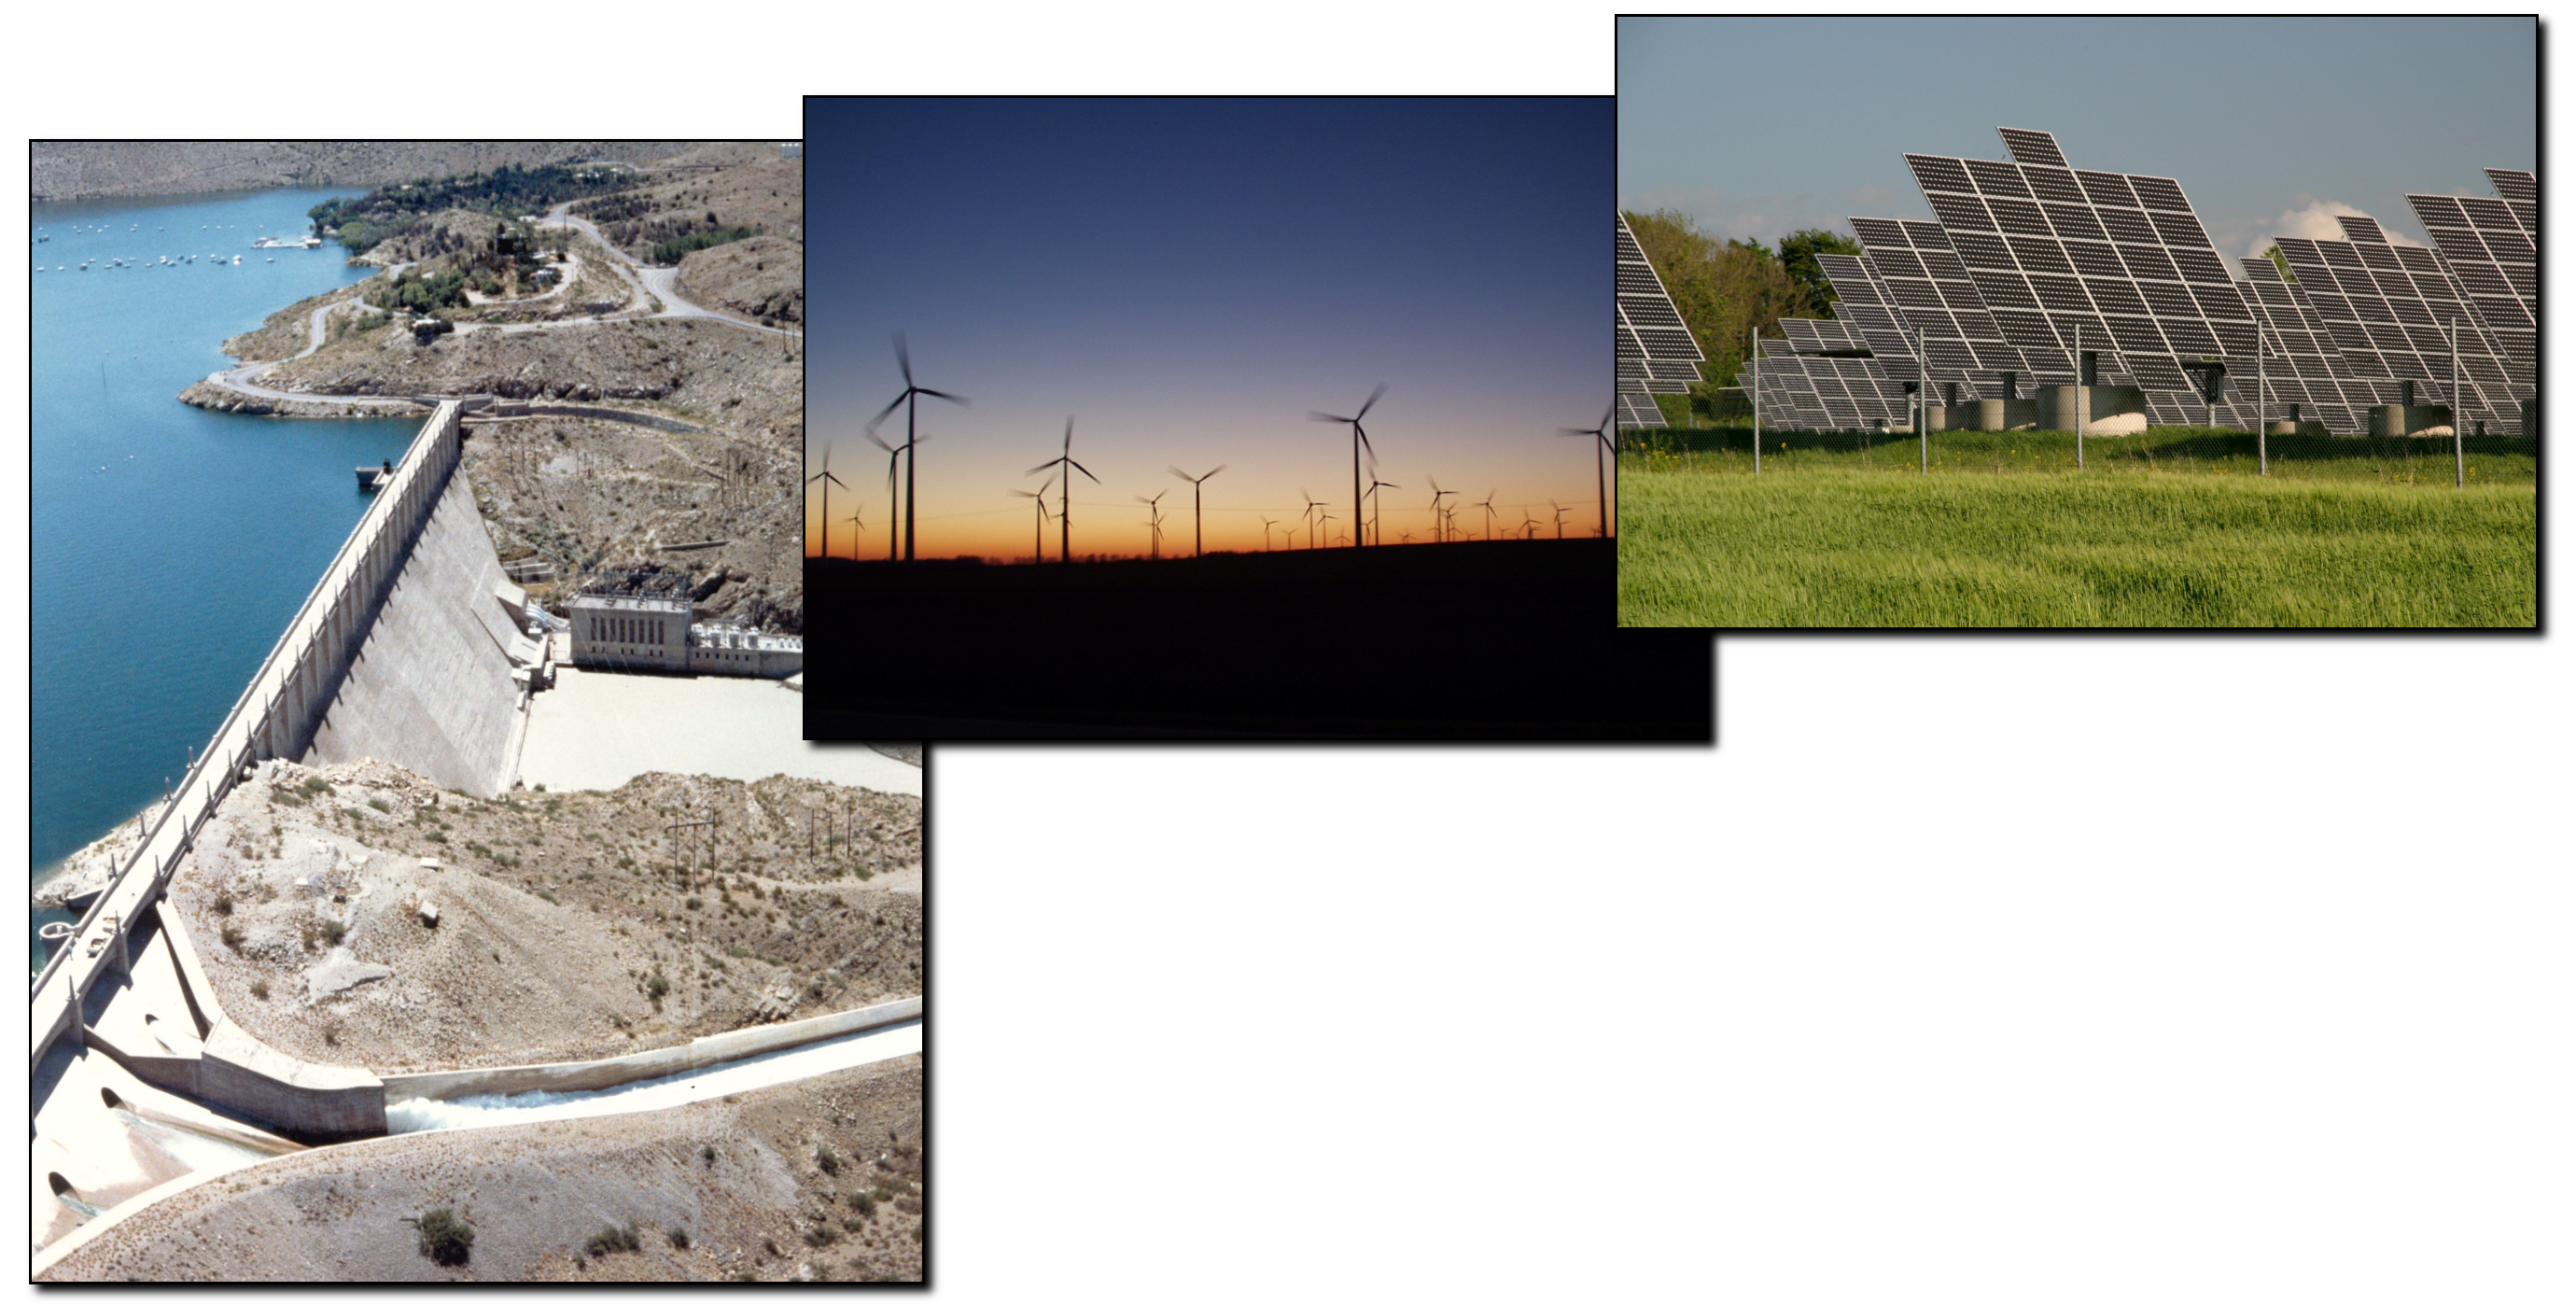
\includegraphics[width=1\textwidth]{pictures/index/index.png}
\end{center}



\newpage

%%%%%%%%%%%%%%%%%%%%%%%%%%
%%%%%%%%Neue Seite%%%%%%%%
%%%%%%%%%%%%%%%%%%%%%%%%%%



\renewcommand{\indexname}{Sachregister}
\addcontentsline{toc}{section}{Sachregister}

\printindex

\end{document}
